\section{Introduction}

This chapter provides a detailed though non-exhaustive description of
the theory and techniques used in this thesis. First is an overview of
Algorithmic Skeletons, GPGPU programming, and the combination of the
two in SkelCL. Second is a description of the machine learning
techniques used in this thesis, followed by the tools and
methodologies used in the evaluation.


\section{Parallel Programming with Algorithmic Skeletons}

Introduced by \citeauthor{Cole1989} in \citeyear{Cole1989},
Algorithmic Skeletons simplify the task of parallel programming by
abstracting common patterns of communication, providing parallel
implementations of higher order functions~\cite{Cole1989}. The
interfaces to generic parallel algorithms exposed by Algorithmic
Skeletons are parameterised by the user with \emph{muscle functions}
that implement problem specific logic. The idea is that this allows
the user to focus on solving the problem at hand, affording greater
ease of use by automating the coordination of parallel resources.


\subsection{Abstracting Task and Data Parallelism}

Algorithmic Skeletons are categorised as either \emph{data} parallel
or \emph{task} parallel. In data parallel skeletons, data is
distributed across nodes for parallel processing across multiple
devices executing a single task. That is, each parallel node executes
the same code, on a unique subset of the data. Examples of data
parallel Algorithmic Skeletons include \emph{map}, \emph{zip}, and
\emph{reduce}. The data parallel operations provided by SkelCL are
described in detail in Section~\ref{sec:skelcl-intro}.

Task parallel skeletons treat the data as a singular object and
instead parallelise the execution of multiple tasks. Tasks are
assigned to threads, which can communicate with each other by passing
data between threads. Examples of task parallel Algorithmic Skeletons
include \emph{pipe}, \emph{task farm}, and \emph{for loops}.


\subsection{Algorithmic Skeleton Frameworks}

\begin{figure}
\centering
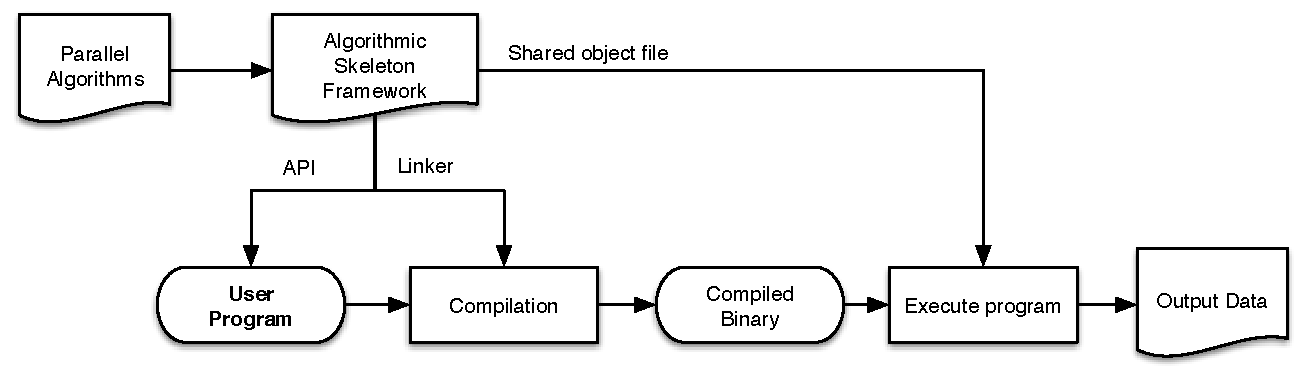
\includegraphics[width=0.99\textwidth]{img/askf}
\caption{%
  Typical usage of a library based Algorithmic Skeleton
  Framework. Other approaches to Algorithmic Skeletons involve
  embedding the API into the core language itself, or using template
  and macro substitution to remove the need for linking with a
  library.%
}
\label{fig:askf}
\end{figure}

Algorithmic Skeleton Frameworks (ASkFs) provide concrete parallel
implementations of a set of parallel patterns, which are parameterised
by the user to generate specific problem solving programs. The
interfaces exposed by frameworks must be sufficiently generic to allow
users to express a range of problems.

Implementations of Algorithmic Skeletons abound, targeting a range of
different use cases and host languages. Notable examples include:
eSkel~\cite{Benoit2005a}, Skandium~\cite{Leyton2010}, and
FastFlow~\cite{Aldinucci2011}. The most prevalent form of ASkF is as a
standalone library built within a host library, which exposes a set of
APIs, shown in Figure~\ref{fig:askf}. See~\cite{Gonzalez2010} for a
more exhaustive review of ASkFs in the research literature.

In industry, Google's MapReduce~\cite{Dean2008} and Intel's Thread
Building Blocks~\cite{IntelTBB} have utilised a similar approach to
abstracting the coordination of parallel resources as in Algorithmic
Skeletons, to great commercial success, although they do not advertise
themselves as such.


\section{GPGPU Programming}

General purpose programming with graphics hardware is a nascent field,
but has shown to enable massive data parallel throughput by
re-purposing the hardware traditionally dedicated to the rendering of
3D graphics for generic computation. This was enabled by hardware
support for programmable shaders replacing the fixed function graphics
pipeline, and support for floating point operations in
2001. \citeauthor{Owens2006} provide a review of the first five years
of general purpose computation on graphics hardware
in~\cite{Owens2006}.

In the ensuing progress towards increasingly programmable graphics
hardware, two dominant programming models have emerged: CUDA and
OpenCL, which both abstract the graphics primitives of GPU hardware
and provide a platform for GPGPU programming. CUDA is a language
developed by NVIDIA for programming their GPUs using a proprietary SDK
and API~\cite{Nvidia2007}, while OpenCL is a vendor-independent open
standard based on a subset of the ISO C99 programming language, with
implementations for devices from most major GPU
manufactures~\cite{Stone2010}. Quantitative evaluations of the
performance of CUDA and OpenCL programs suggest that performance is
comparable between the two systems, although the wider range of target
architectures for OpenCL means that appropriate optimisations must be
made by hand or by the compiler~\cite{Komatsu2010,Karimi2010}.


\subsection{The OpenCL Programming Model}

\begin{figure}
\centering
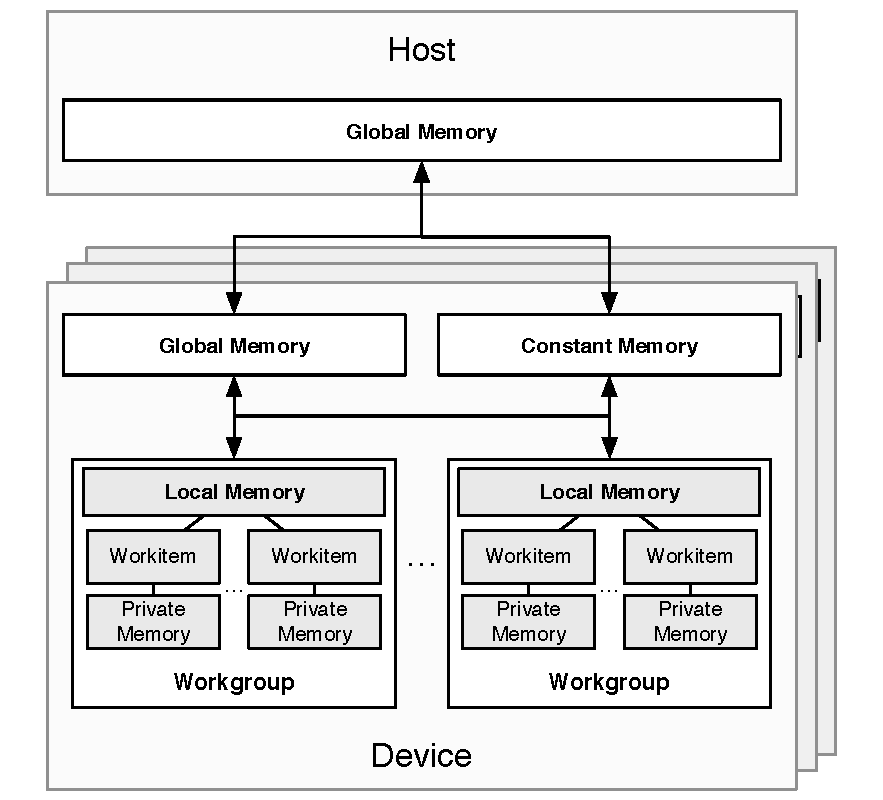
\includegraphics[width=0.5
\textwidth]{img/opencl-memory}
\caption{%
  The OpenCL memory model. The host communicates with each device
  through transfers between global memory spaces. The capacity of each
  type of memory is dependent on the device hardware. In general,
  private memory is the fastest and smallest, and global memory is the
  largest and slowest.%
}
\label{fig:opencl-memory}
\end{figure}

OpenCL is a parallel programming framework which targets CPUs, GPUs,
and other parallel processors such as Field-Programmable Gate
Arrays. It provides a set of APIs and a language (based on an extended
subset of C) for controlling heterogeneous \emph{compute devices} from
a central host. Programs written for these devices are called
\emph{kernels}, and are compiled by platform-specific toolchains. When
a kernel is to be executed, each unit of computation is referred to as
a \emph{workitem}, and these work items are bunched into
\emph{workgroups}. For GPUs, workgroups execute on the Single
Instruction Multiple Data (SIMD) processing units in lockstep. This
can cause a severe performance penalty for flow control across
workgroups, as ``thread masks'' must be used to stall the execution of
workitems across diverging branches.

The wide range of supported execution devices and differing
standard-compliant implementations makes portable performance tuning
of OpenCL programs a difficult task~\cite{Rul2010}, and the
interactions between optimisations and the hardware are complex and
sometimes counter-intuitive~\cite{Ryoo2008}.


\subsubsection{Memory Model}

Unlike the flat memory model of CPUs, OpenCL uses a hierarchical
memory model. The host and each OpenCL device has a single global
memory address space. Each workgroup has a local memory space, and
each workitem has a region of private memory.

Workgroups cannot access the memory of neighbouring workgroups, nor
can workitems access the private memory of other workitems. OpenCL
provides synchronisation barriers to allow for communication between
workitems within a single workgroup via the local memory, but not
global barriers. Memory transfers between the host and devices occurs
between global memory regions. In the case of programming
heterogeneous devices, these transfers must occur over the connection
bus between the CPU and device (e.g.\ PCIe for discrete GPUs), which
typically creates a performance bottleneck by introducing a
performance overhead to transfer data to the device for processing,
than back to the device afterwards. Direct transfers of data between
devices is not supported, requiring an intermediate transfer to the
host memory.

\subsubsection{GPU vs CPU performance analysis}

% V. W. Lee, P. Hammarlund, R. Singhal, P. Dubey, C. Kim, J. Chhugani,
% M. Deisher, D. Kim, A. D. Nguyen, N. Satish, M. Smelyanskiy, and
% S. Chennupaty, “Debunking the 100X GPU vs. CPU myth,” ACM SIGARCH
% Comput. Archit. News, vol. 38, p. 451, 2010.
In~\cite{Lee2010}, \citeauthor{Lee2010} present a performance analysis
of optimised throughput computing applications for GPUs and CPUs. Of
the 14 applications tested, they found GPU performance to be
$0.7\times$-$14.9\times$ that of multi-threaded CPU code, with an
average of only 2.5$\times$. This is much lower than the
$100\times$-$1000\times$ values reported by other studies,
% TODO: ^^ Citation needed!
a fact that they attribute to uneven comparison of optimised GPU code
to unoptimised CPU code, or vice versa. \citeauthor{Lee2010} found
that multithreading, cache blocking, reordering of memory accesses and
use of SIMD instructions to contribute most to CPU performance. For
GPUs, the most effective optimisations are reducing synchronization
costs, and exploiting local shared memory. In all cases, the programs
were optimised and hand-tuned by programmers with expert knowledge of
the target architectures. It is unclear whether their performance
results still hold for subsequent generations of devices.


% Enmyren, J., & Kessler, C. (2010). SkePU: a multi-backend skeleton
% programming library for multi-GPU systems. In Proceedings of the
% fourth international workshop on High-level parallel programming and
% applications (pp. 5–14). ACM. Retrieved from
% http://dl.acm.org/citation.cfm?id=1863487
\subsubsection{Skeletal Programming for GPUs}

\TODO{%
  SkePU Similar to SkelCL in scope and ambition, alternative
  implementation with C++ macros and CUDA~\cite{Enmyren2010}.%
}


\section{High-Level GPU Programming with SkelCL}\label{sec:skelcl-intro}

Introduced in~\cite{Steuwer2011}, SkelCL is an object oriented C++
library that provides OpenCL implementations of data parallel
algorithmic skeletons for heterogeneous parallelism using CPUs or
multi-GPUs. SkelCL addresses the parallel programmability challenge by
allowing users to easily harness the power of GPUs and CPUs for data
parallel computing~\cite{Steuwer2011}. To achieve this, SkelCL
separates the concerns of problem solving and coordinating
heterogeneous devices, achieving this abstraction using Algorithmic
Skeletons.

Skeletons are parameterised with muscle functions by the user, which
are compiled into OpenCL kernels for execution on device hardware. The
Vector and Matrix container types transparently handle communication
between the host and device memory, and support partitioning for
multi-GPU execution.

SkelCL is freely
available\footnote{\url{http://skelcl.uni-muenster.de}} and
distributed under dual GPL and academic licenses.



\TODO{%
  Towards high-level programming~\cite{Steuwer2012}. Support for
  multi-GPU systems~\cite{Steuwer2013a}. Stencil
  computations~\cite{Breuer2014}. Allpairs
  skeleton~\cite{Steuwer2014}. An example of reduced programmer effort
  for real world application using SkelCL: \cite{Steuwer2013}%
}


\subsection{Pattern definitions}

\TODO{Brief descriptions and example uses of patterns.}

\subsubsection{Map}

\begin{equation}
\map\left(f, [x_1,x_2,\ldots,x_n]\right) \to [f(x_1),f(x_2),\ldots,f(x_n)]
\end{equation}

When applied to an $n \times m$ matrix:

\begin{equation}
\map\left(f,
\begin{bmatrix}
  x_{11} & \cdots & x_{1m} \\
  \vdots & \ddots & \vdots \\
  x_{n1} & \cdots & x_{nm}
\end{bmatrix}\right)
\to
\begin{bmatrix}
  f(x_{11}) & \cdots & f(x_{1m}) \\
  \vdots & \ddots & \vdots \\
  f(x_{n1}) & \cdots & f(x_{nm})
\end{bmatrix}
\end{equation}

\subsubsection{Zip}

\begin{equation}
\zip\left( \oplus, [x_1,x_2,\ldots,x_n], [y_1,y_2,\ldots,y_n] \right)
\to
\left[ x_1 \oplus y_1, x_2 \oplus y_2, \ldots, x_n \oplus y_n \right]
\end{equation}

\begin{equation}
\begin{split}
\zip \left( \oplus,
\begin{bmatrix}
  x_{11} & \cdots & x_{1m} \\
  \vdots & \ddots & \vdots \\
  x_{n1} & \cdots & x_{nm}
\end{bmatrix},
\begin{bmatrix}
  y_{11} & \cdots & y_{1m} \\
  \vdots & \ddots & \vdots \\
  y_{n1} & \cdots & y_{nm}
\end{bmatrix} \right) \\
\to
\begin{bmatrix}
  x_{11} \oplus y_{11} & \cdots & x_{1m} \oplus y_{1m} \\
  \vdots & \ddots & \vdots \\
  x_{n1} \oplus y_{n1} & \cdots & x_{nm} \oplus y_{nm}
\end{bmatrix}
\end{split}
\end{equation}

\subsubsection{Reduce}

\begin{equation}
\reduce \left( \oplus, i, [x_1,x_2,\ldots,x_n] \right)
\to
x_1 \oplus x_2 \oplus \ldots \oplus x_n
\end{equation}

\begin{equation}
\reduce \left( \oplus, i,
\begin{bmatrix}
  x_{11} & \cdots & x_{1m} \\
  \vdots & \ddots & \vdots \\
  x_{n1} & \cdots & x_{nm}
\end{bmatrix} \right)
\to
x_{11} \oplus x_{12} \oplus \ldots \oplus x_{nm}
\end{equation}

\subsubsection{Scan}

\begin{equation}
\scan \left( \oplus, i, [x_1,x_2,\ldots,x_n] \right)
\to
\left[ i, x_1, x_1 \oplus x_2, \ldots, x_1 \oplus x_2 \oplus \ldots \oplus x_n \right]
\end{equation}

\subsubsection{AllPairs}

\begin{equation}
\allpairs \left( \oplus,
\begin{bmatrix}
  x_{11} & \cdots & x_{1d} \\
  \vdots & \ddots & \vdots \\
  x_{n1} & \cdots & x_{nd}
\end{bmatrix},
\begin{bmatrix}
  y_{11} & \cdots & y_{1m} \\
  \vdots & \ddots & \vdots \\
  y_{n1} & \cdots & y_{nm}
\end{bmatrix} \right)
\to
\begin{bmatrix}
  z_{11} & \cdots & z_{1m} \\
  \vdots & \ddots & \vdots \\
  z_{n1} & \cdots & z_{nm}
\end{bmatrix}
\end{equation}

where:

\begin{equation}
z_{ij} =
\left[ x_{i1}, x_{i2}, \ldots, x_{id} \right] \oplus
\left[ y_{j1}, y_{j2}, \ldots, y_{jd} \right]
\end{equation}

An additional implementation is provided for when the $\oplus$
operator is known to match that of a zip pattern:

\begin{equation}
z_{ij} =
\left[
  x_{i1}, \oplus y_{j1}, x_{i2} \oplus y_{j2}, \ldots, x_{id} \oplus y_{jd}
\right]
\end{equation}


\subsubsection{Stencil}

\TODO{Define border region (sometimes referred to as halo region).}

Stencils are patterns of computation which operate on uniform grids of
data, where the value of each cell is updated based on its current
value and the value of one or more neighbouring elements, called the
border region. In SkelCL, a 2D stencil skeleton allows users to
provide a function which updates a cell's value, and SkelCL
orchestrates the parallel execution of this function across all
cells. Each cell maps to a single work item; and this collection of
work items is then divided into \emph{workgroups} for execution on the
target hardware.

In SkelCL, the border region is described by a \emph{stencil shape},
which defines an $i \times j$ rectangular region about each cell which
is used to update the cell value. Stencil shapes may be asymmetrical,
and a defined in terms of the number of cells in the border region to
the north, east, south, and west of each cell, shown in
Figure~\xref{\TODO{Diagram of 3 stencil shapes.}}

Given a customising function $f$, a stencil shape $S$, and an
$n \times m$ matrix:

\begin{equation}
\stencil \left( f, S,
\begin{bmatrix}
  x_{11} & \cdots & x_{1m} \\
  \vdots & \ddots & \vdots \\
  x_{n1} & \cdots & x_{nm}
\end{bmatrix} \right)
\to
\begin{bmatrix}
  z_{11} & \cdots & z_{1m} \\
  \vdots & \ddots & \vdots \\
  z_{n1} & \cdots & z_{nm}
\end{bmatrix}
\end{equation}

where:

\begin{equation}
z_{ij} = f \left(
\begin{bmatrix}
  z_{i-S_n,j-S_w} & \cdots & z_{i-S_n,j+S_e} \\
  \vdots & \ddots & \vdots \\
  z_{i+S_s,j-S_w} & \cdots & z_{i+S_s,j+S_e}
\end{bmatrix} \right)
\end{equation}

A popular application of Stencil codes is for iterative problems, in
which \todo{\ldots} discrete time steps $0 <= t <= t_{max}$, and
$t \in \mathbb{Z}$

\begin{equation}
g(f, S, M, t) =
\begin{cases}
  \stencil \left( f, S, g(f, S, M, t-1) \right),& \text{if } t \geq 1\\
  M_{init}, & \text{otherwise}
\end{cases}
\end{equation}

A Stencil operation in which the size of the stencil shape $S$ is zero
in every direction is functionally equivalent to a Map operation.

\TODO{Explain border handling logic\ldots Add a diagram of the 3
  border handling techniques.}


\subsection{Container Types}

\TODO{Description of vector and matrices, supported data types, lazy
  data transfer \ldots}

\subsubsection{Data distributions}

\TODO{Description and diagrams for single, block, copy, and overlap
  distributions.}


\subsection{Implementation Details}

Each skeleton is represented by a template class, declared in a header
file detailing the public API. A private header file contains the
template definition. E.g. \texttt{SkelCL/Map.h} contains the Map
class, and \texttt{SkelCL/detail/MapDef.h} contains the
implementation. Non-trivial kernels are stored in separate source
files, e.g. \texttt{SkelCL/detail/MapKernel.cl}.

\TODO{Description of OpenCL skeleton templates, and the compilation
  process - i.e. substitution of user functions, handling additional
  arguments  \ldots}

\TODO{Algorithm listing for stencil}


\subsubsection{Stencil}

% TODO: This listing isn't required.
\lstinputlisting[
  language=C++,
  float,
  floatplacement=t,
  label=lst:skelcl-stencil-interface,
  caption={
    Interface for SkelCL stencil skeleton.
  }
]{dat/skelcl-stencil-interface.cpp}


\subsubsection{StencilSequence}

\TODO{Iterative stencils, and sequences of stencils}


\subsection{Example Application}

\TODO{%
  Provide definition of an example stencil program, a code listing for
  SkelCL implementation, and a comparison of runtimes using a decent
  GPU vs. sequential CPU. Preferably also hand coded OpenCL?%
}


\subsection{Workgroup size and Stencil Codes}

% TODO:

In OpenCL, kernels are mapped to work-items for execution on the
processing units of GPUs and CPUs. These work-items are then grouped
into one or more workgroups. The choice of workgroup size is left to
the developer, but with two sets of constraints. The first set of
constraints is the maximum workgroup size which an execution device
supports. This value cannot be exceeded, irrespective of the kernel
being executed. The second constraint is the maximum workgroup size a
kernel supports, and can only be queried at runtime once a kernel has
been compiled. The selection of workgroup size for stencil skeletons
is particularly relevant to the performance of the stencil as it
affects utilisation of fast local memory. In a stencil code, each
work-item reads the values of multiple neighbouring elements. To
facilitate this, the value of all elements within a workgroup are
stored in fast local memory, which greatly reduces the read latency
for GPUs. Changing the workgroup size affects the amount of local
memory required for each workgroup, which in turn affects the number
of workgroups which may be simultaneously active. \TODO{Explain (or
  rephrase) why this isn't a curve that gets better as the memory size
  goes up until a threshold after which it falls off. Would binary
  search work?}

\TODO{%
  While the user is clearly in control of the type of work which is
  executed, the size of the grid, and the size of the border region,
  it is very much the responsibility of the skeleton implementation to
  select what workgroup size to use. As such I designed an experiment
  to explore just what effect changing workgroup sizes has on the
  performance of Stencil skeletons.%
}

\TODO{Add diagram showing workgroup decomposition.}


\section{Machine Learning}


\subsubsection{ZeroR}


\subsection{Classification}


\subsubsection{Naive Bayes}


\subsubsection{Random Forest}


\subsubsection{Logistic Regression}


\subsubsection{Support Vector Machines}


\subsubsection{Decision Trees}


\subsection{Regression}


\subsubsection{Linear Regression}


\subsubsection{Random Forest}


\section{Validation and Testing}


\subsubsection{Cross-validation}


\section{Statistics}

A number of statistical tools are used throughout this thesis to
ensure.

\subsubsection{Statistical Testing}

Student's \emph{t}-test


\subsubsection{Confidence Intervals}

95\% confidence intervals are calculated assuming a Gaussian
distribution of runtimes (given our sample size of
$n \ge 30$~\cite{Georges2007}):

\begin{align}
\bar{x} &= \frac{1}{n}\sum_{i=1}^{n} x_i\\
\sigma &= \sqrt{\frac{\sum_{i=1}^{n}(x_i - \bar{x})^2}{n - 1}}\\
c_1 &= \bar{x} - z_{1-\alpha/2}\frac{\sigma}{\sqrt{n}}\\
c_2 &= \bar{x} + z_{1-\alpha/2}\frac{\sigma}{\sqrt{n}}
\end{align}


\subsubsection{Histogram}

Histograms are a widely used statistical visualisation which shows the
distribution of numerical data. The data is first divided into a set
of discrete, equally sized sub-intervals, or \emph{bins}. The number
of data points in each bin is used to show visualise the density
distribution. The shortcoming of histograms is that their appearance
is heavily influenced by three user-selected parameters: the number of
bins, the width of bins (binwidth), and the endpoints chosen. As such,
they may provide a misleading representation of the data if
inappropriate values for any of these parameters are chosen. Kernel
Density estimation is a technique for showing the distribution of data
which circumvents some of these issues.


\subsubsection{Kernel Density Estimation}

A Kernel Density Estimate (KDE) is an approximation of the probability
density function of a random variable. Given a random variable $x$,
and bandwidth $h$ and a kernel $K$, the KDE $\hat{f}_h(x)$ can be
found using:

\begin{equation}
  \hat{f}_h(x) = \frac{1}{nh} \sum^{n}_{i=1} K\left( \frac{x - x_i}{h} \right)
\end{equation}

Using a smooth kernel such as a Gaussian distribution for the kernel
produced a smooth density estimated, unlike histograms. However, like
histograms, the appearance of a Kernel Density Estimate plot is
dependent on the value of the bandwidth parameter $h$ (equivalent to
binwidth in histograms), so care must be taken to select a value to
minimise over or under smoothing. Grouped data can be shown by
plotting multiple KDEs on the same axes, although if the number of
groups is large, a box plot or violin plot may be more appropriate.


\subsubsection{Box plot}

Box plots are used to show the distribution of quartile ranges for
grouped data. The contain the following features:

\begin{itemize}
\item Horizontal lines at the lower quartile, median and upper
  quartile.
\item Vertical lines above and below the upper and lower quartiles to
  the most extreme data point within 1.5 IQR of the upper/lower
  quartile, with horizontal whiskers at the end of the vertical lines.
\item Dots beyond the ends of the vertical lines to show outliers.
\end{itemize}

A variation of box plots used in this thesis is the violin plot, which
extends the box plot with a fitted Kernel Density Estimate plot to
show the probability \emph{density} of data at different values. To
construct a violin plot, KDEs for each group are rotated and mirrored
to generate a smoothed visualisation of the distribution.


\section{Summary}
